In this section we present our main results for the detectable LISA DCO population in our fiducial model. We find that on average, a 4-year LISA mission will detect about \BHBHFourYear{} BHBHs, \BHNSFourYear{} BHNSs and \NSNSFourYear{} NSNSs (c.f.\ Table~\ref{tab:detection_rates}). We first show the distribution of the sources together with the sensitivity curve in Section~\ref{sec:dcos_on_sc}, before exploring the parameter distributions for detectable sources in Section~\ref{sec:fiducial_distributions} and the measurement uncertainties in Section.~\ref{sec:measurement_uncertainties}.

\subsection{Distribution on the sensitivity curve}\label{sec:dcos_on_sc}

\begin{figure*}[p]
    \centering
    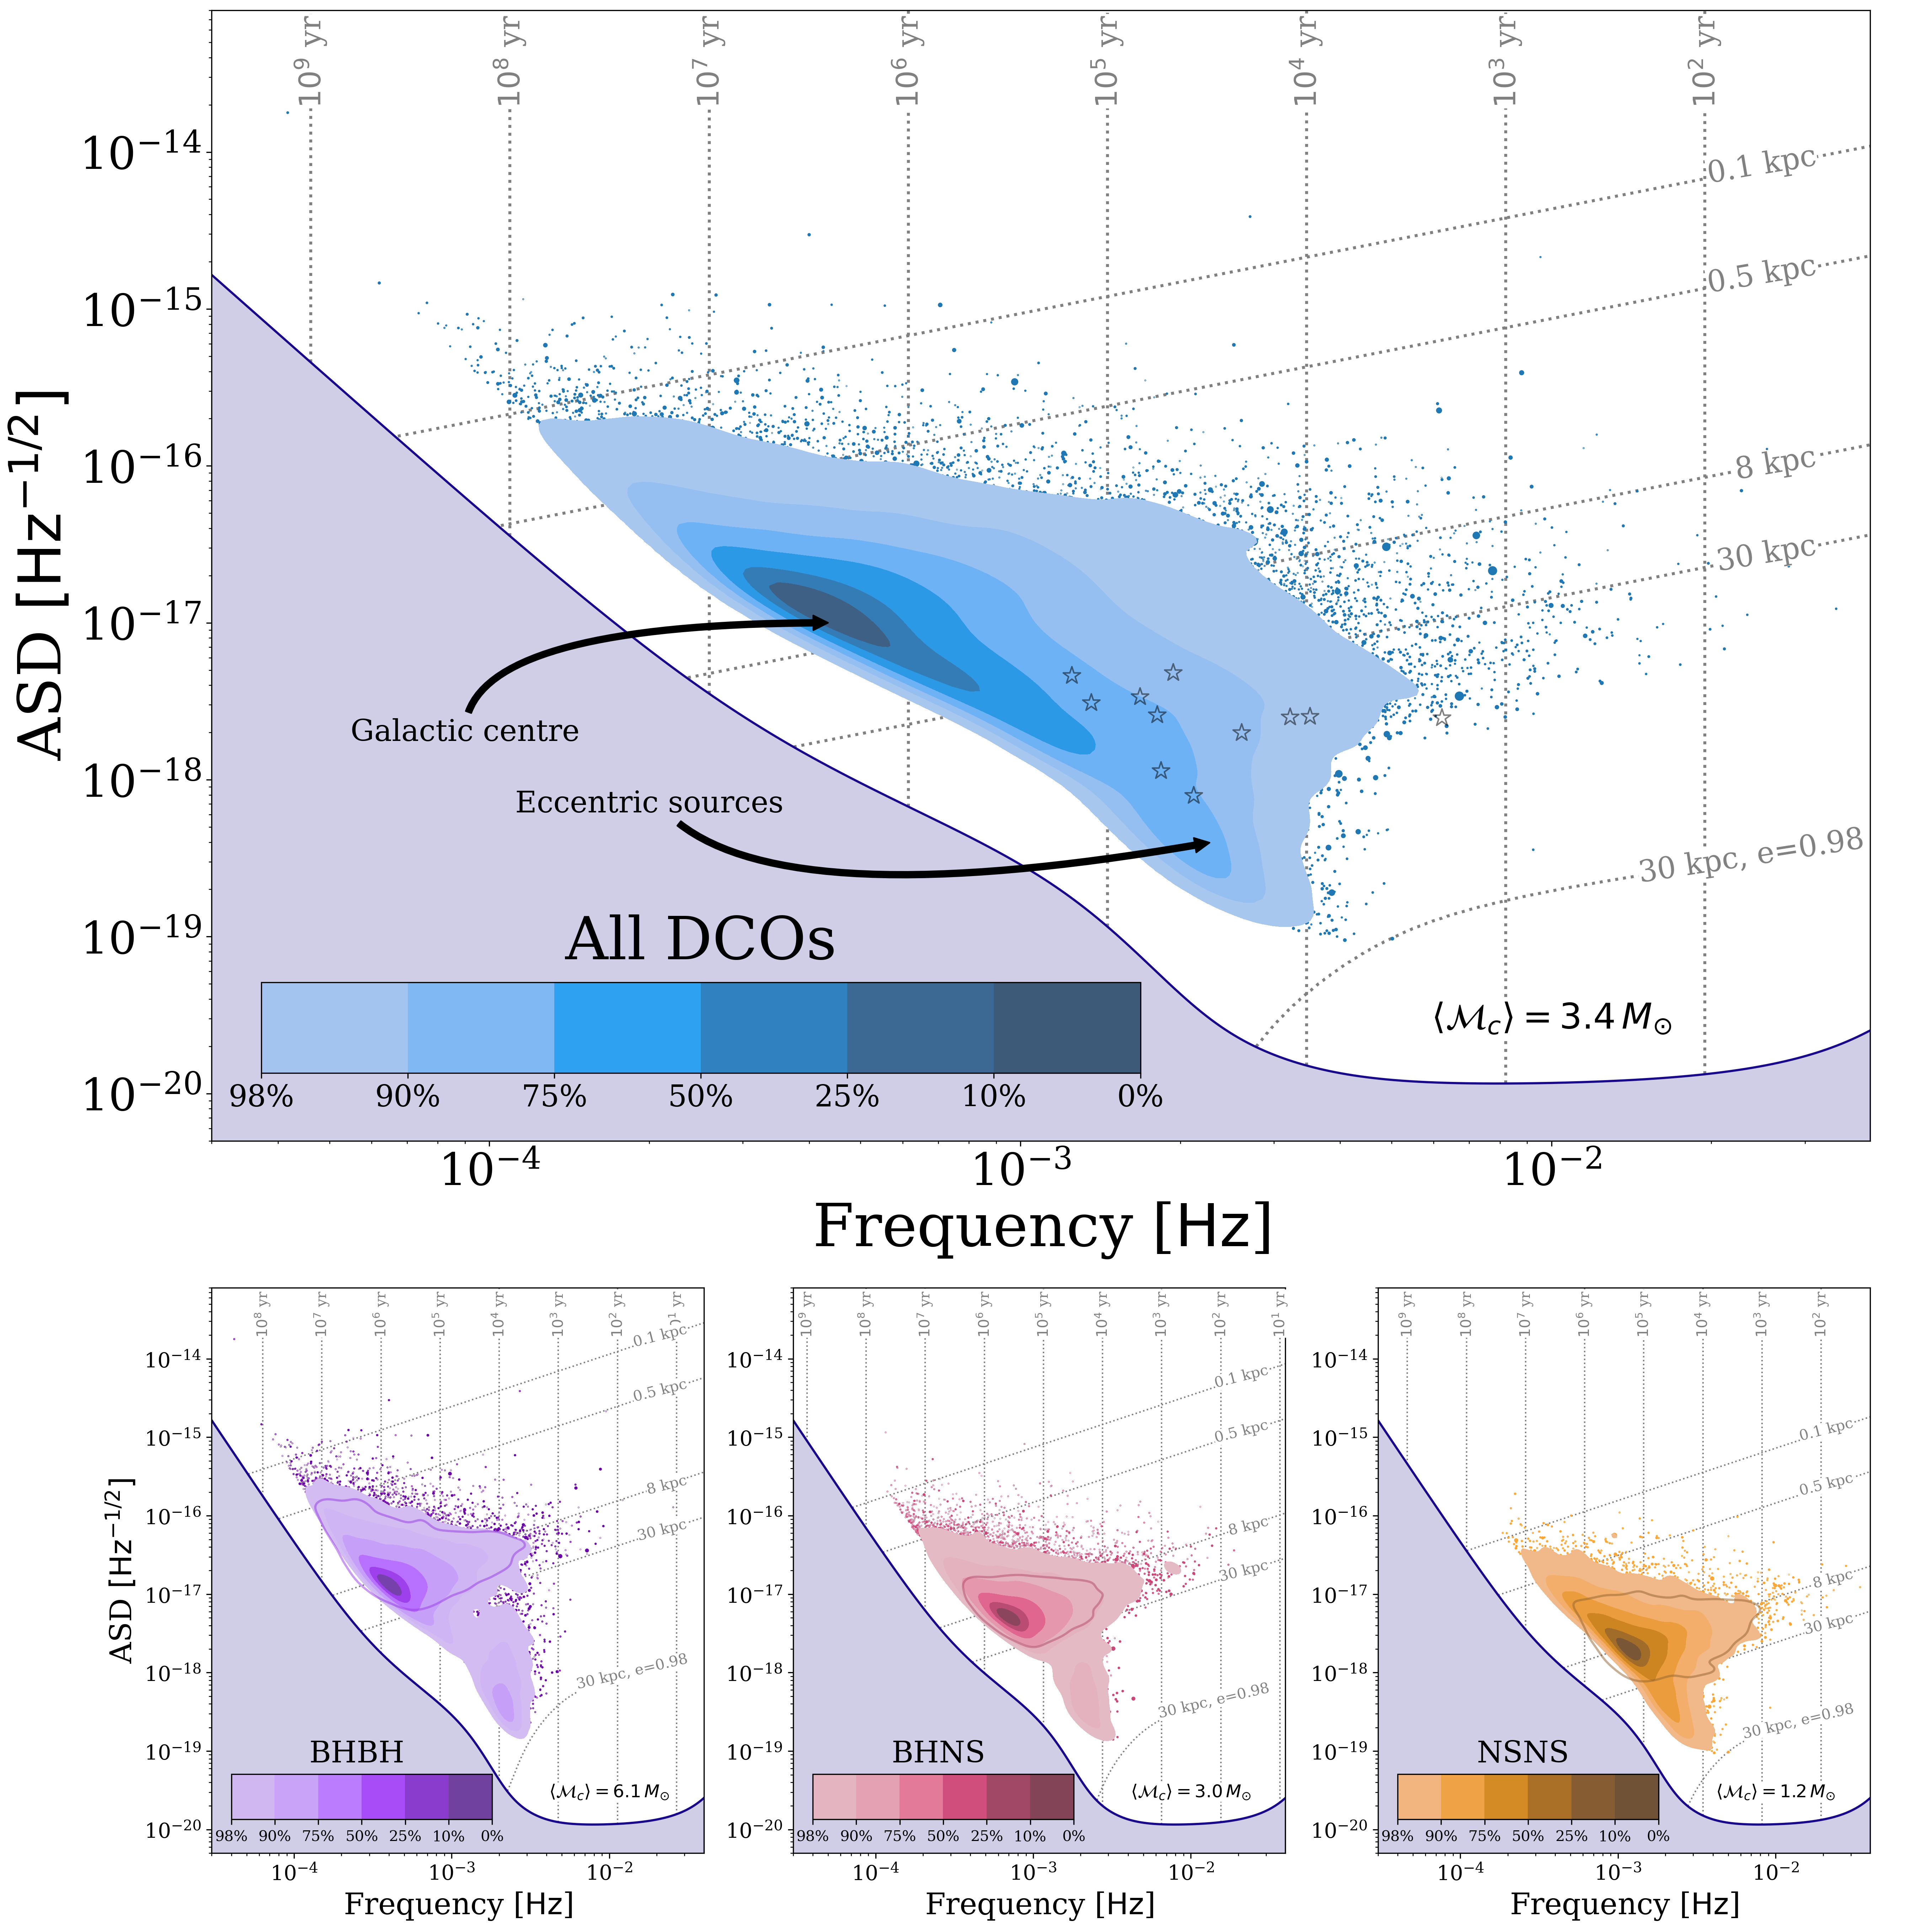
\includegraphics[width=\textwidth]{2_dcos_on_sc.png}
    \caption{Density distribution of detectable BHBH, BHNS and NSNS binaries are shown together with the LISA sensitivity curve. In the top panel we show all systems with the LISA verification binaries over plotted (star symbols, \citealp{Kupfer+2018}). In the bottom panels we separate by type. Contours show the percentage of the population enclosed. The remaining 2\% of the population is shown as dots with a size that scales with the sampling weight. For reference we show lines where a circular binary of average chirp mass $\avg{\mathcal{M}_c}$ would reside for a given remaining inspiral time (vertical lines) and distance (diagonal line). To highlight the role of eccentricity we further show the signal expected for an eccentric binary at 30 kpc. The coloured line in the bottom panels shows a contour that encloses 90\% of the population that is circular. See Sec.~\ref{sec:dcos_on_sc} for a discussion.}
    \label{fig:dcos_on_sc}
\end{figure*}

We show the expected distribution of detectable DCOs together with the LISA sensitivity curve in Figure~\ref{fig:dcos_on_sc}. This shows that the detectable population of these DCOs is concentrated at comparatively lower frequencies than the LISA verification binaries (shown as stars in the top panel). This is expected since producing the same SNR as a BHBH, BHNS or NSNS with a relatively lower mass (circular) WDWD requires a higher frequency. This finding is in agreement with \citet{Sesana+2020} and as noted in that work, this could possibly be used to distinguish more massive DCOs from WDWDs probabilistically. There are several other notable features in these distributions. To understand these we overplot reference lines indicating where a circular binary with the average chirp mass ($\avg{\mathcal{M}_c}$, annotated in each panel) would reside for a given remaining inspiral time (vertical lines) and a given distance (diagonal lines).

Firstly, we note that the peak of the density distribution coincides with the centre of the Milky Way as expected, since binaries are most likely to be formed towards the centre of the Galaxy. Additionally, we expect that if a population is entirely circular, it should be bounded approximately between the $0.1$--$30 \unit{kpc}$ lines, roughly the minimum and maximum distance to a source in the Milky Way. From inspection of the bottom panels with each individual DCO type we see that this is the true for a large fraction of the population. However, there is a distinct subpopulation of binaries that extend downwards, especially around $2 \unit{mHz}$. This offshoot is composed of eccentric binaries for which the circular distance contours do not apply. For illustrative purposes, we plot the 90\% contour of only the \textit{circular} sources in our sample over the density distribution in each of the bottom panels and this subsample is indeed bounded by $0.1$--$30 \unit{kpc}$ the distance lines. We also plot a line of constant distance at $30 \unit{kpc}$ for an eccentric binary with $e = 0.98$ to show the different limit for eccentric sources. To further illustrate this point, we show the same plot but with each point coloured by its eccentricity in Fig.~\ref{fig:dcos_on_sc_ecc_col}. Overall, we can see that eccentric sources tend to be located on a slightly different location on the sensitivity curve and so this could perhaps be used help in identifying them.

We plot vertical lines that give the inspiral time for a circular binary with the average chirp mass (annotated in each panel). From these lines we can understand the trend of the density distribution decreasing with increasing frequency. Sources with higher frequencies have shorter inspiral times and thus DCOs will spend less time in these regimes, meaning that more sources are detected at lower frequencies. Note that these inspiral time lines should only be used as guidelines for the population as a whole, as the inspiral time of each individual source will be a function of its mass and eccentricity. It is also evident for each DCO source that the tail of the high frequency sources is more numerous near to the Galactic centre than at short distances. This is simply because there are more sources in the galactic centre and so the chances of `catching' a binary at high frequency are better.

\subsection{Properties of the detectable systems}\label{sec:fiducial_distributions}

In Figure~\ref{fig:fiducial_pdf_distributions}, we show the distribution of the individual parameters of the population of detectable binaries and discuss the various features in the following sections.

\subsubsection{Orbital Frequency}
The orbital frequency distributions for BHBHs, BHNSs and NSNSs peak at progressively increasing frequencies. This is because a higher mass DCO at the same distance and eccentricity requires a lower frequency to produce the same signal-to-noise ratio and thus be detected. The BHBH distribution has a tail that extends to $8 \times 10^{-6} \unit{Hz}$, which is comprised of highly eccentric binaries. These systems are still detectable by LISA as the high eccentricity means that the majority of the GW signal is emitted at higher harmonics at higher frequencies that are located in the LISA band. Similar tails are not as prevalent for BHNSs and NSNSs as they do not have as many eccentric binaries.

\begin{figure*}[t]
    \centering
    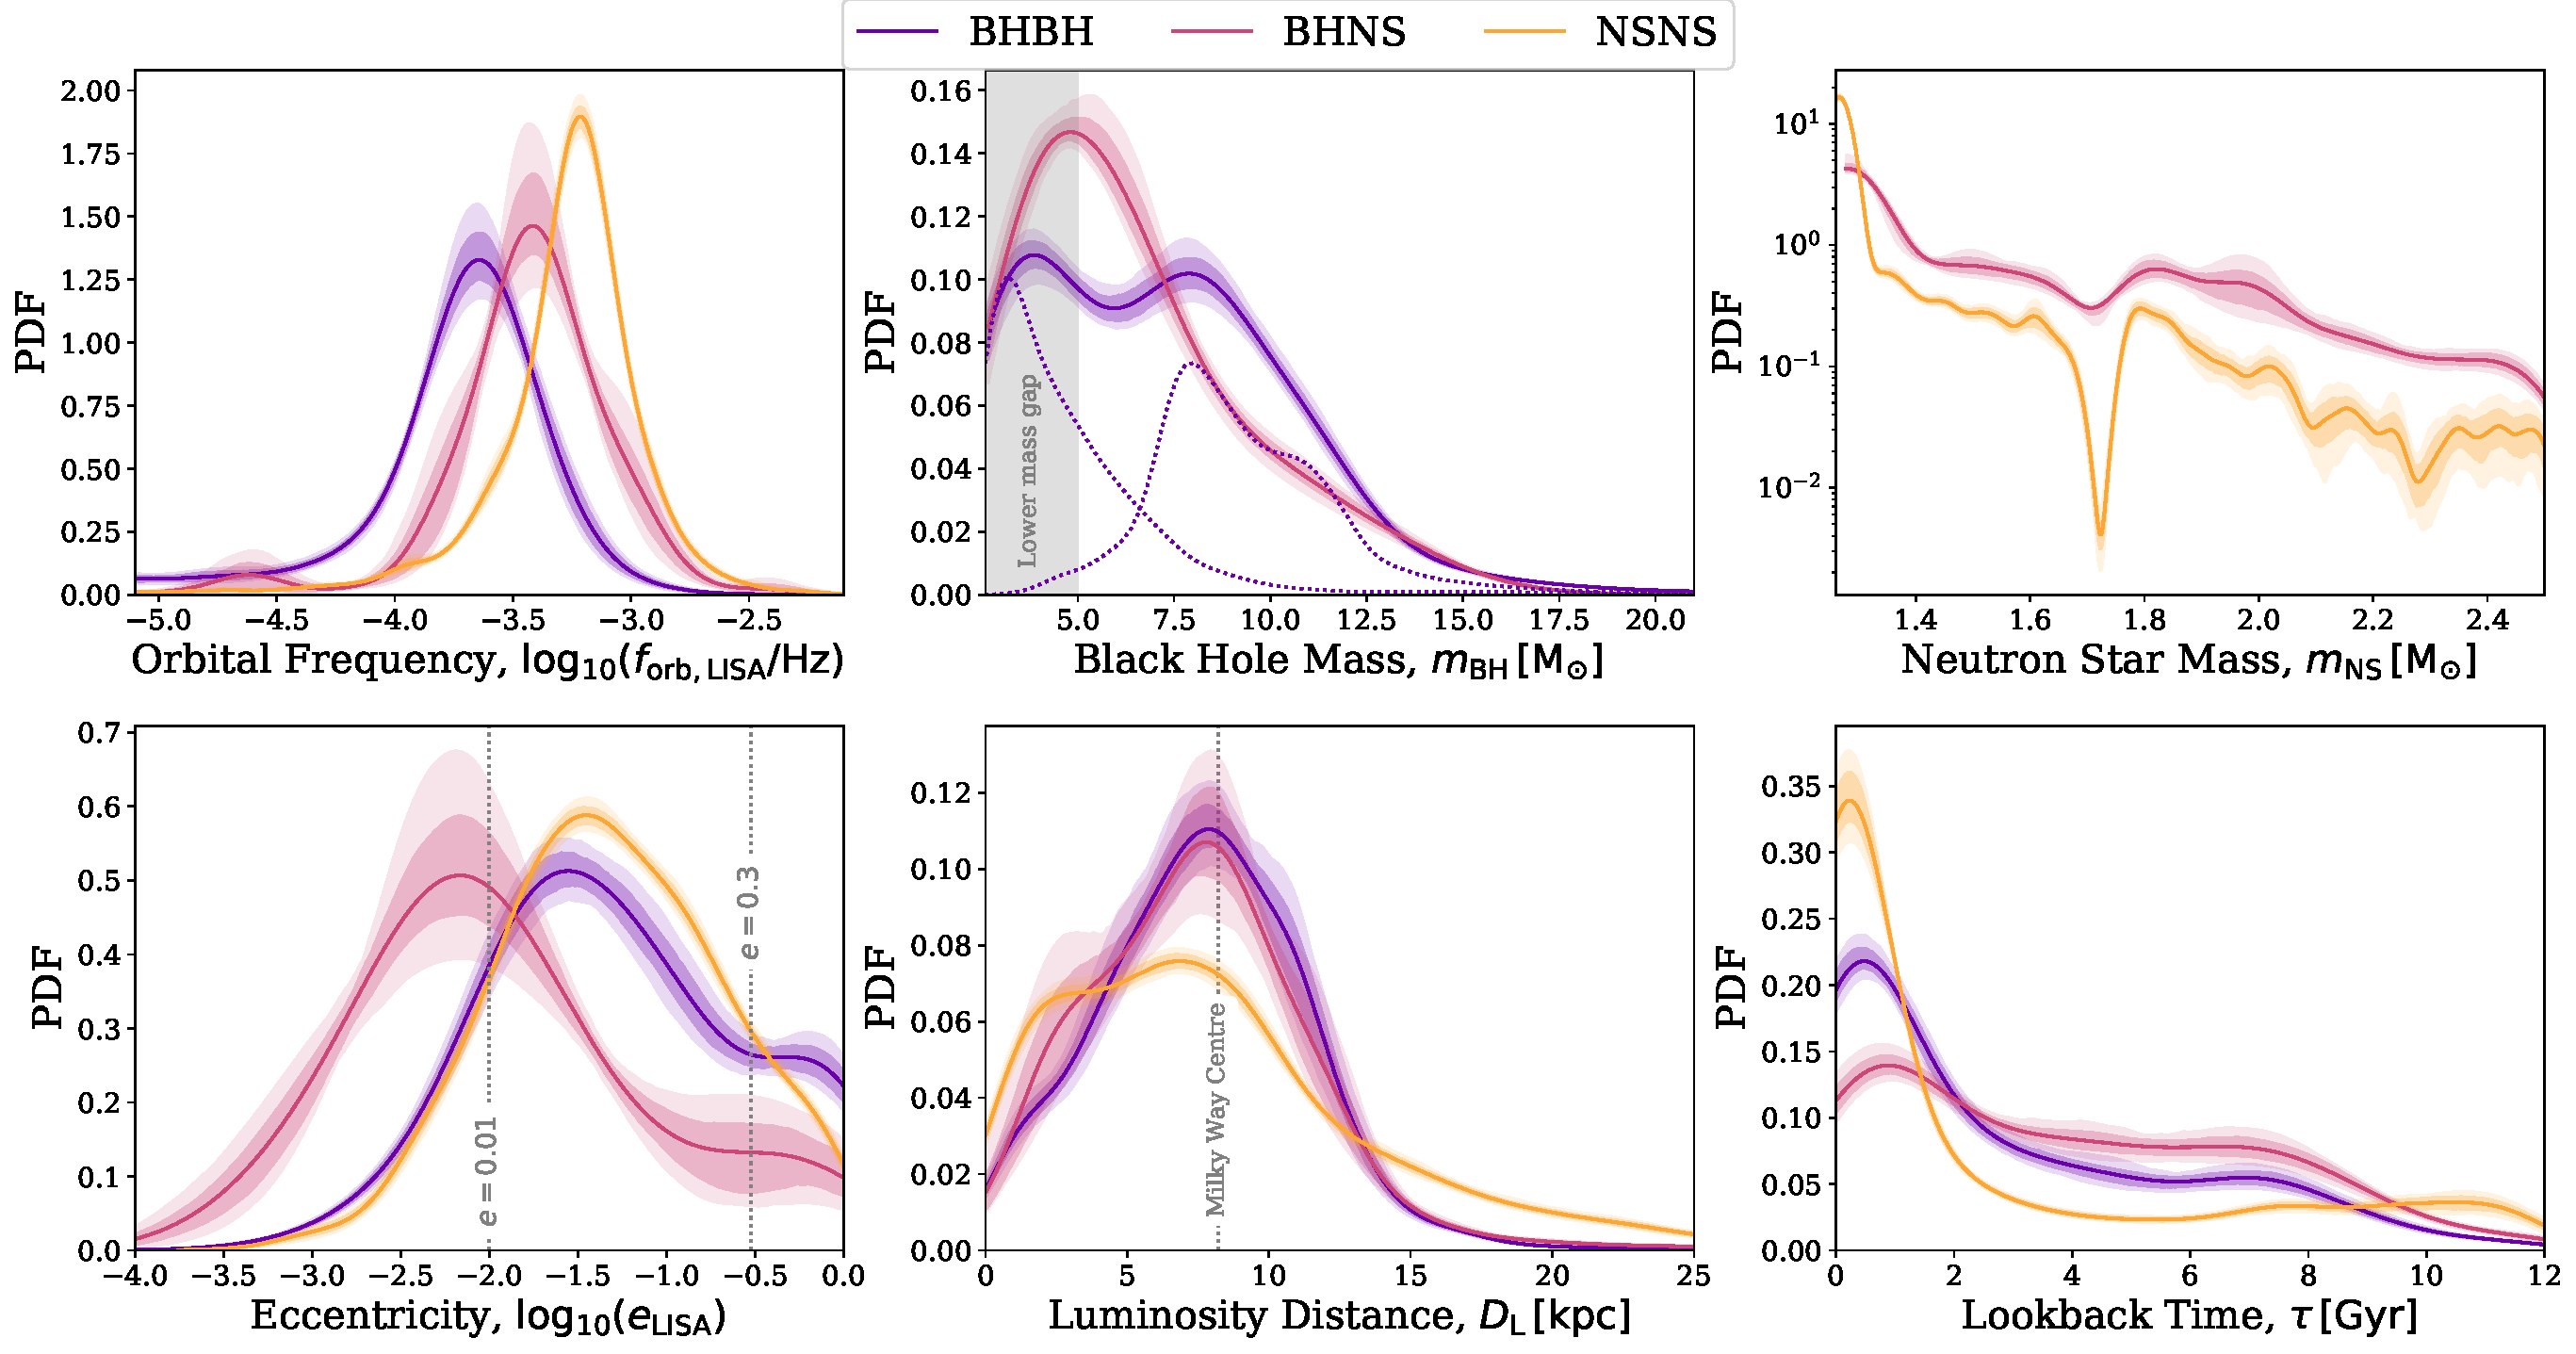
\includegraphics[width=\textwidth]{4_detectable_properties_4yr.pdf}
    \caption{Properties of detectable systems for a 4-year LISA mission in our fiducial model. Each panel shows a kernel density estimator for a single property, coloured by DCO type. The shaded areas show the 1- and 2-$\sigma$ uncertainties (obtained via bootstrapping). The dotted lines in the black hole mass panel show the individual primary and secondary mass distributions. See Sec.~\ref{sec:fiducial_distributions} for a discussion.}
    \label{fig:fiducial_pdf_distributions}
\end{figure*}

\subsubsection{Black Hole Mass}
For both the BHBHs and BHNSs, the black hole mass distribution extends to relatively low masses, with $\BHBHmBHBelowEleven{}$ and $\BHNSmBHBelowEleven{}$ respectively below $11 \unit{M_{\odot}}$. Unlike ground-based detectors, LISA is not biased to higher masses and so the mass distribution more closely follows the IMF. In addition, at the high metallicities in the Milky Way, stellar winds are much stronger and strip away much of the stellar mass before BH formation, resulting the less massive black holes. The mass distribution extends down to $2.5 \unit{M_{\odot}}$, our fiducial maximum neutron star mass. Since the \citet{Fryer+2012} \textit{delayed} remnant mass prescription (applied in this work) does not produce a mass gap between neutron stars and black holes. Indeed we expect $\BHBHLowerMassGap{}$ and $\BHNSLowerMassGap{}$ of detected BHBH and BHNS systems to contain a black hole in the lower mass gap. Therefore, LISA could help to confirm or rule out the existence of the lower mass gap.

The bimodality of the BHBH distribution is a result of unequal mass ratios. The two peaks are from the primary and secondary black hole masses, which peak around $8 \unit{M_{\odot}}$ and $3.5 \unit{M_{\odot}}$ respectively. We show these individual distributions as dotted curves below the main BHBH distribution.

\subsubsection{Mass Ratio}
The mass ratio distribution for each DCO type is relatively distinct from the others. The majority of NSNSs have a mass ratio close to unity, with $\NSNSqAbovePointEight{}$ of systems having $q > 0.8$. The reason for the concentration around equal masses is that most NSs are formed either through electron-capture supernovae or from low mass stars. We set the remnant mass for any system formed through ECSN to $1.26 \unit{M_{\odot}}$ (see Sec.~\ref{sec:fiducial_physics}). The remnant mass prescription that we use gives a fixed fallback mass for any star with a CO core mass less than $2.5 \unit{M_\odot}$, such that many NSs are given the identical mass of $1.278 \unit{M_\odot}$ in the \textit{delayed} prescription \citep[see][Eq.~19]{Fryer+2012}. This means that many NSs are formed with equal masses and hence we see a mass ratio distribution peaked around unity.

In contrast, only $\BHBHqAbovePointEight{}$ of detectable BHBHs are formed with $q > 0.8$ and distribution peaks around $q = 0.4$. The reasoning for these unequal mass ratio systems is as follows: in order to produce a BHBH, most formation channels require at least the first mass transfer to be stable. This stability is strongly dependent on the mass ratio such that equal mass ratios (at the moment of mass transfer) are preferred for creating BHBHs. Yet, since stellar winds are so strong at high metallicity, and even stronger for more massive stars, the primary star will experience significant mass loss and so an initially \textit{unequal} mass ratio is preferred so that the masses are more balanced at the first instance of mass transfer. Since mass transfer occurs after the end of the main sequence for most of our BHBHs, the star will have a well defined core and these core masses, which go on to form BHs, will reflect the initially unequal mass ratios.

We find that detectable BHNSs have even more unequal mass ratios, such that the distribution is almost entire disjoint from that of NSNSs. Moreover, the mass ratio distribution is bimodal, where the two peaks arise from two distinct formation scenarios. Around two thirds of detectable BHNSs experience at least one common envelope event, whilst the last third are formed through only stable mass transfer. The first peak at $q = 0.18$ is from systems that experience at least one CE and occurs at the expected mass ratio, which approximately follows the mean BH mass ($\sim 6.5 \unit{M_\odot}$) and NS mass ($\sim 1.2 \unit{M_\odot}$). Yet we also see a second peak at higher mass ratios around $q = 0.34$, which arise from the fraction of the population that underwent only stable mass transfer. The stability of mass transfer is strongly dependent on the mass ratio and thus these systems have a bias for more equal mass ratio systems, leading to a peak at higher $q$.

\subsubsection{Eccentricity}
The eccentricity distributions show that detectable BHBHs are most likely to be highly eccentric of the three DCOs. This may seem counter-intuitive since neutron stars receive stronger natal kicks, which cause the orbit to become eccentric. However, these stronger kicks often result in disrupted or too-wide binaries in the more weakly bound NSNSs. In contrast, BHBHs can receive strong kicks that impart high eccentricity without disrupting and thus tend to be more eccentric. This effect is compounded by the fact that we can see BHBHs at lower orbital frequencies, meaning that they have not had as much time to circularise and so still have significant eccentricity by the time of the LISA mission.

An eccentricity of $e = 0.01$ is the lower bound on the measurable eccentricity with LISA proposed by \citet{Nishizawa+2016}. We find that a significant fraction of DCOs ($\BHBHNotCirc{}$ of BHBHs, $\BHNSNotCirc{}$ of BHNSs and $\NSNSNotCirc{}$ of NSNSs) exceed this bound. This is in contrast to several previous work that assume all DCOs are circular once they reach the LISA mission \citep[e.g.][]{Lamberts+2018, Sesana+2020}. Moreover, we find that $\BHBHHighlyEccentric{}$, $\BHNSHighlyEccentric{}$ and $\NSNSHighlyEccentric{}$ of BHBHs, BHNSs and NSNSs respectively have $e > 0.3$. At this eccentricity the majority of the gravitational wave power is emitted in higher harmonics above the orbital frequency and thus the signal would appear at higher frequencies in LISA.

\subsubsection{Time since formation}
The progenitors of Galactic DCOs in our sample are formed throughout the history of the Milky Way, with more formed at earlier times (see Fig.~\ref{fig:galaxy_schematic}). In contrast, we find that the \textit{detectable} systems are primarily formed recently, with the majority formed in the past $2 \unit{Gyr}$, in addition to a tail of systems out to earlier times.

The peak at recent times is due to the fact that most binaries in our sample are formed with merger times on the order of a couple of Gyr (since most form through a common envelope phase that significantly tightens the binary). For a binary to be in the LISA band and detectable it must be near the end of its inspiral and so LISA will be most sensitive to sources that were formed a couple of Gyr ago.

The peak is sharpest for NSNSs as they have the highest orbital frequencies and largest fraction of eccentric system, which result in shorter inspiral times and therefore later formation times. Conversely, the peak is less prominent for BHNSs as they are the most circular, have moderate orbital frequencies and masses.

\subsubsection{Time until merger}
The final panel of Fig.~\ref{fig:fiducial_pdf_distributions} shows the remaining time until merger for each of the DCO types at the start of LISA mission. The distributions are strikingly similar and peak with merger times of around a Myr.

The merger time is a function of the mass, frequency and eccentricity of the sources, such that more massive, higher frequency and more eccentric sources merge faster \citep[][Eq.~5.14]{Peters+1964}. So, despite the fact that each DCO type often has higher values in any one of these properties, the convolution of all three tends to negate the differences. For example, NSNSs have the highest orbital frequencies and are mildly eccentric whilst BHNSs have moderate orbital frequencies and are more circular. However, BHNSs are more massive in general and so the overall merger times are distributed very similarly for both DCO types.

\subsection{Distribution in the Milky Way}\label{sec:mw_detectable_distribution}
In the first panel of Fig.~\ref{fig:detectable_distance_dist} we show the distribution of the luminosity distance of detectable systems. Each DCO's luminosity distance distribution peaks around $8 \unit{kpc}$ since this is the distance to the centre of the Milky Way and thus the most dense location of DCOs. There is a bias in each distribution for systems at lower distances since closer binaries are easier to detect. This bias is most prominent for the NSNS distribution since, on average, their lower relative masses require a smaller distance in order to be detected.

However, more surprisingly, we also see that the NSNS distribution extends to higher distances than the other DCOs. The reason for this is that the NSNS population has the highest fraction of ``mildly'' eccentric systems ($0.01 < e < 0.3$). The BHNS population has a much higher fraction of effectively circular systems ($e < 0.01$), which emit weaker gravitational wave compared to equivalent eccentric systems. Therefore, despite their relatively higher masses, the maximum distance at which a source is detectable is generally lower than the eccentric NSNSs and hence the distribution tends to zero at smaller distances. Conversely, the BHBH population has a higher fraction of \textit{high} eccentricity systems $e > 0.3$. Although one may naively expect that this would result in stronger signals (and so further distances), for a system to have these high eccentricities in LISA, it must still be early in its evolution and thus have a low orbital frequencies. The result of this is that high eccentricity systems tend to have lower SNRs and so cannot be detected at large distances. Overall we see that the eccentricity distribution of NSNSs occupies a ``sweet spot'' where the gravitational wave power is increased compared to circular systems, but it isn't too high that the frequency is significantly impacted. This means that NSNSs can be seen out to the largest distances of the three DCO types.

In the lower panel of Fig.~\ref{fig:detectable_distance_dist}, we show the density distribution for detectable DCOs in the galaxy. We see that most sources are concentrated in the Galactic center, with a bias towards to the position of the Sun. Yet we also show that systems are detectable out to the edges of the galaxy and this is especially true for NSNSs.

\begin{figure}[thb]
    \centering
    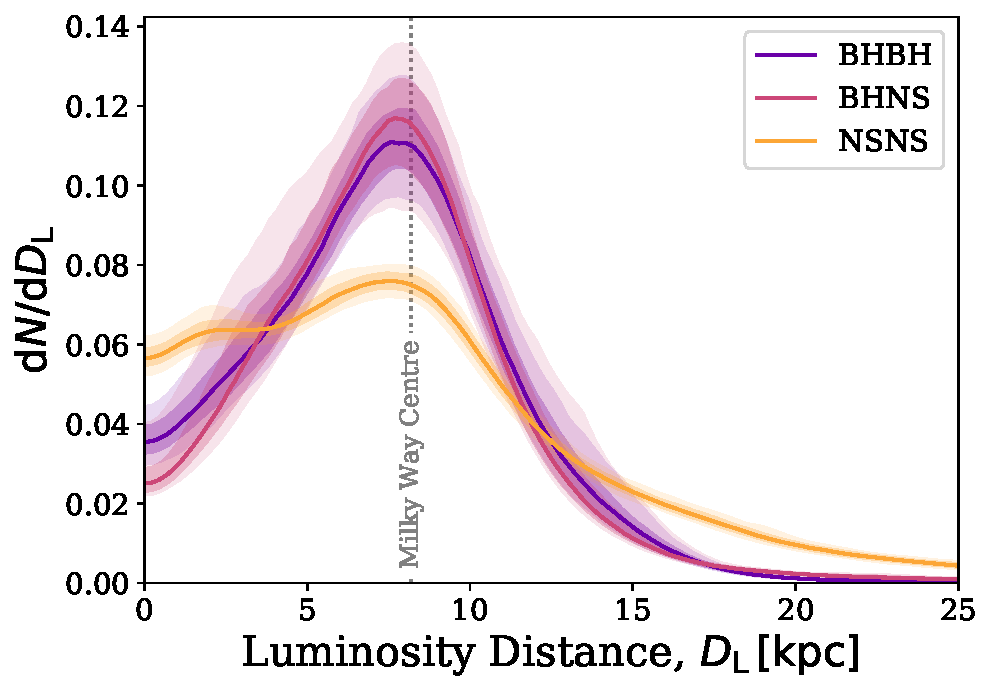
\includegraphics[width=\columnwidth]{detectable_distance_distribution_4yr.pdf}
    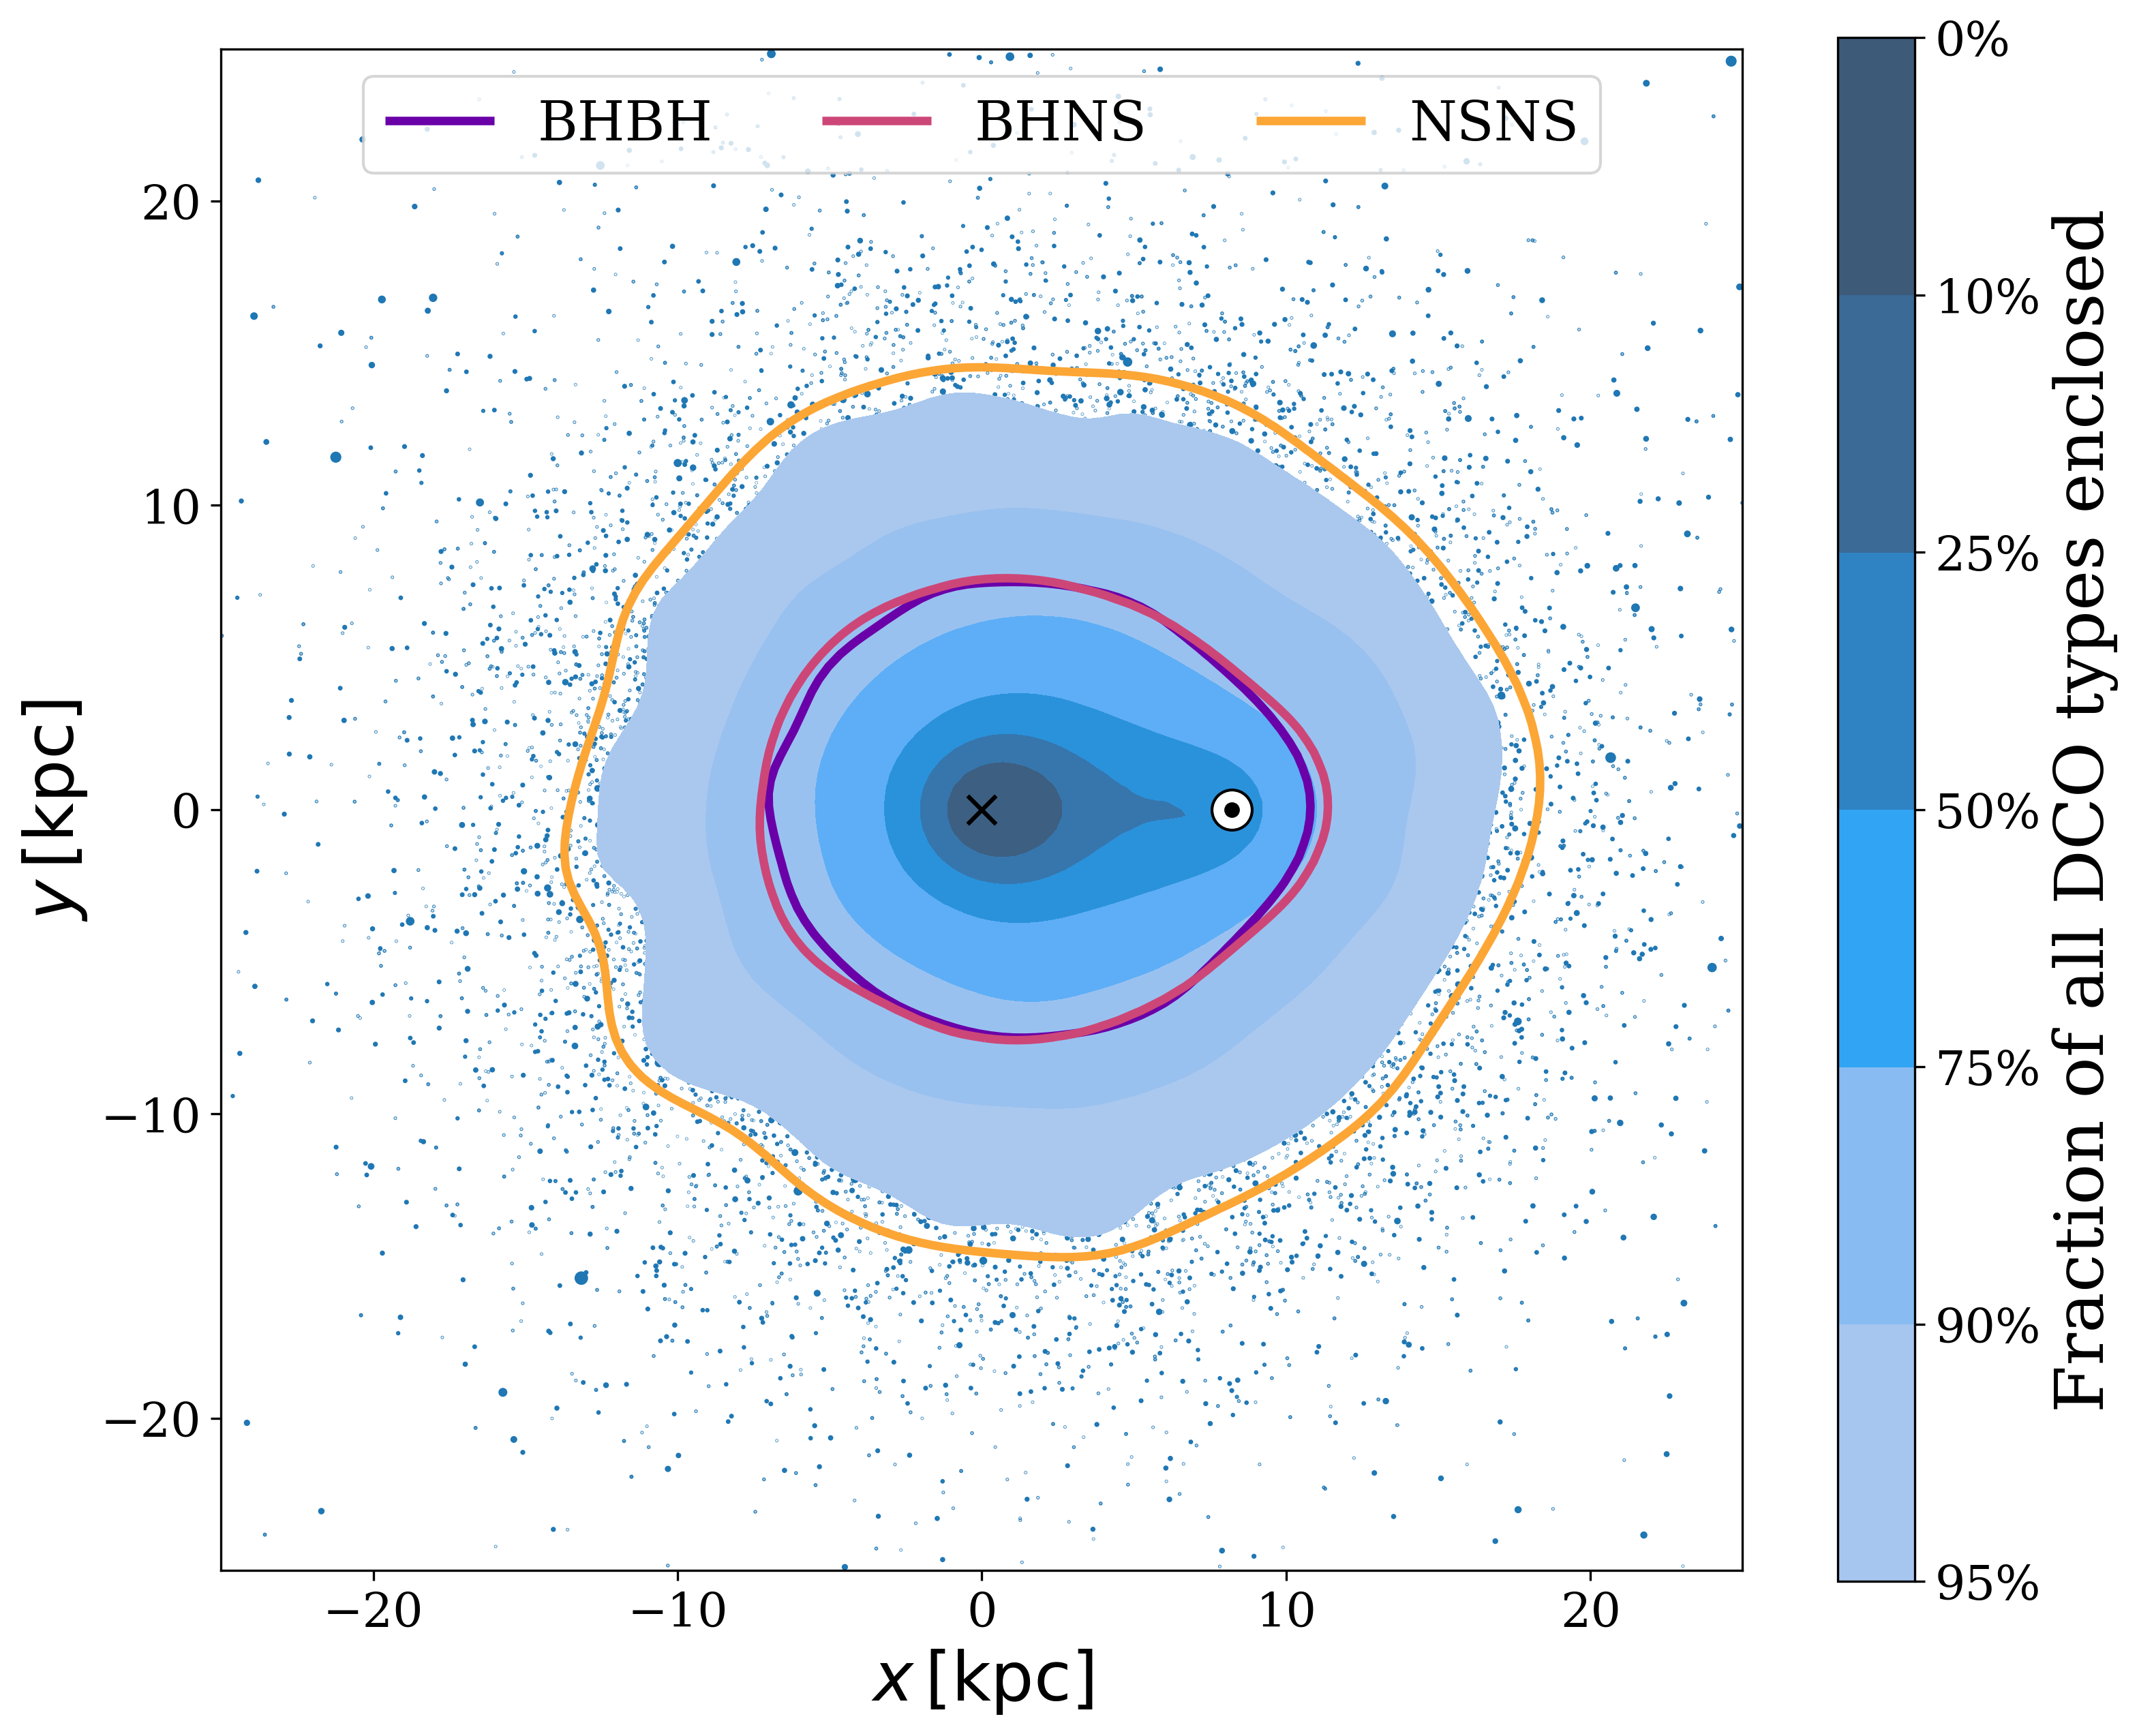
\includegraphics[width=\columnwidth]{galaxy_density_distribution.png}
    \caption{\textbf{Top:} As Figure~\ref{fig:fiducial_pdf_distributions}, but for the luminosity distance. \textbf{Bottom:} A face-on view of the Galactic density distribution for detectable DCOs. We only show the density distribution for the top 95\% of the sources, the rest are indicated by scatter points whose sizes correspond to their STROOPWAFEL weights. The coloured lines show the 90\% contour for each of the individual DCO types. The `x' shows the centre of the galaxy, whilst the $\odot$ shows the position of the Sun.}
    \label{fig:detectable_distance_dist}
\end{figure}

\subsection{Measurement Uncertainties}\label{sec:measurement_uncertainties}
Although it is useful to investigate the underlying parameters of the detectable population, it is also important to consider what LISA will actually \textit{measure} during a detection.

\subsubsection{Chirp mass uncertainty}

The chirp mass uncertainty is important for identifying the source of a GW signal. It is calculated using the uncertainty on the orbital frequency, the time derivative of the orbital frequency and the eccentricity. This is because the chirp mass can be written as
\begin{equation}
    \mathcal{M}_c = \frac{c^3}{G} \left( \frac{5 \pi}{48 n} \frac{\dot{f}_{n}}{F(e)} \right)^{3/5} \frac{1}{(2 \pi f_{\rm orb})^{11/5}},
\end{equation}
where $f_{\rm orb}$ is the orbital frequency, $\mathcal{M}_{c}$ is the chirp mass (defined in Eq.~\ref{eq:chirp_mass}), $e$ is the eccentricity and
\begin{equation}
    F(e) = \frac{1 + \frac{73}{24} e^2 + \frac{37}{96} e^4}{(1 - e^2)^{7/2}},
\end{equation}
is the enhancement factor of gravitational wave emission for an eccentric binary over an otherwise identical circular binary \citep[][Eq.~17]{Peters+1963}. Therefore the chirp mass uncertainty is
\begin{equation}\label{eq:chirp_mass_uncertainty}
    \qty( \frac{\Delta \mathcal{M}_c}{\mathcal{M}_c} )^2 = \left( \frac{11}{5} \frac{\Delta f_{\rm orb}}{f_{\rm orb}} \right)^2 + \left( \frac{3}{5} \frac{\Delta \dot{f}_{\rm dom}}{\dot{f}_{\rm dom}} \right)^2 + \left( \frac{3}{5} \frac{\Delta F(e)}{F(e)} \right)^2,
\end{equation}
where $f_{\rm dom}$ is the harmonic frequency with the strongest SNR ($f_{\rm dom} = n_{\rm dom} f_{\rm orb}$ and $n_{\rm dom} = 2$ for circular binaries) as this will provide the best measurement.

We calculate the frequency uncertainties using \citet{Takahashi+2002}, such that
\begin{align}\label{eq:f_orb_unc}
    \frac{\Delta f_{\rm orb}}{f_{\rm orb}} &= 4 \sqrt{3} \cdot \frac{1}{\rho} \frac{1}{T_{\rm obs}} \frac{1}{f_{\rm orb}}, \\
    \frac{\Delta \dot{f}_{\rm dom}}{\dot{f}_{\rm dom}} &= 6 \sqrt{5} \cdot \frac{1}{\rho} \left(\frac{1}{T_{\rm obs}} \right)^2 \frac{1}{\dot{f}_{\rm dom}},
\end{align}
where $\rho$ is the signal-to-noise ratio and $T_{\rm obs}$ is the LISA mission length. We calculate the eccentricity certainty, $\Delta e$, following the methods of \citet{Lau+2020} and \citet{Korol+2021}, which use the relative SNRs of different harmonics to work out the eccentricity. We propagate this uncertainty such that
\begin{equation}
    \frac{\Delta F(e)}{F(e)} = \Delta e \cdot \frac{(1256 + 1608 e^2 + 111 e^4) e}{96 + 196 e^2 - 255 e^4 - 37 e^6}.
\end{equation}

We use Eq.~\ref{eq:chirp_mass_uncertainty} to calculate the chirp mass uncertainty for each DCO in our sample and plot it in Fig.~\ref{fig:m_c_unc}. We find that approximately $\BHBHChirpMassMeasureable{}$ BHBHs, $\BHNSChirpMassMeasureable{}$ BHNSs and $\NSNSChirpMassMeasureable{}$ NSNSs have measurable chirp masses (as indicated by the shaded region). This uncertainty is generally dominated by the uncertainty on the time derivative of the frequency, since most of the binaries are too early in their inspiral for LISA to measure a strong chirp.

\begin{figure}[ht]
    \centering
    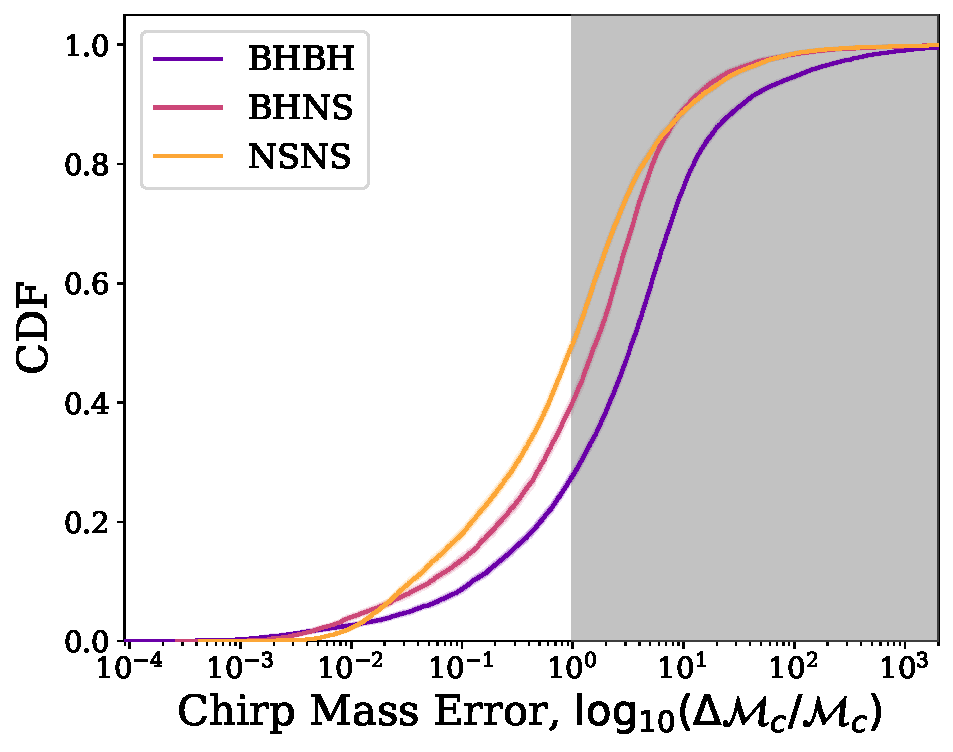
\includegraphics[width=\columnwidth]{chirp_mass_uncertainty_4yr.pdf}
    \caption{Cumulative distribution function for error on the chirp mass. Colours indicate DCO type and shading shows 1- and 2-$\sigma$ uncertainties (obtained via bootstrapping). Shaded region indicates region with unmeasureable chirp mass.}
    \label{fig:m_c_unc}
\end{figure}

\subsubsection{Sky localisation}
We quantify the sky localisation of a source by calculating its angular resolution. Since we find that all potential sources are stationary on the timescale of the LISA mission, following \citet{Mandel+2018}, we can use the timing accuracy of LISA and the effective detector baseline to calculate the angular resolution, $\sigma_{\theta}$, as
\begin{equation}
    \sigma_{\theta} = 16.6^\circ \left(\frac{7}{\rho}\right) \left(\frac{5 \times 10^{-4} \unit{Hz}}{f_{\rm dom}}\right) \left( \frac{2 \unit{AU}}{L} \right),
\end{equation}
where $L$ is the effective detector baseline, which for LISA is 2 AU since it will orbit the Sun.

We plot the angular resolution in Fig.~\ref{fig:ang_res}. The area of a patch on the sky that can be attributed to a source is given by $A = \pi \sigma_\theta^2$. From this plot, we see that the majority of sources can be resolved to an angular resolution of 10 degrees. The size of a pencil beam for a 15m diameter SKA dish observing at 1.4 GHz is roughly 0.67 square degrees, corresponding to an angular resolution of $\sigma_\theta = \sqrt{(0.67 / \pi)} = 0.46^\circ$ (which, for intuition, is approximately the angular size of the moon). Applying this to the plot shows that about 10-20\% of DCOs can be covered by a single pointing of SKA. However, since these LISA sources are essentially stationary in frequency space, observations need not be limited to a single pointing. We will discuss the prospects of matching LISA detections to radio pulsars with SKA further in Sec.~\ref{sec:pulsar_matching}.

\begin{figure}[ht]
    \centering
    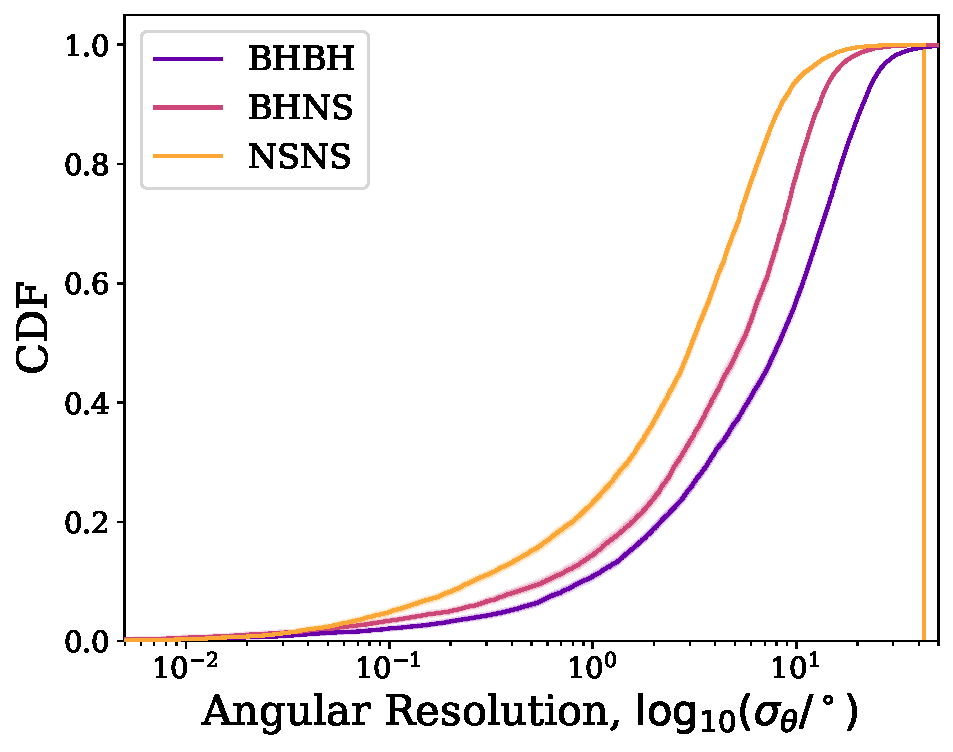
\includegraphics[width=\columnwidth]{angular_resolution_4yr.pdf}
    \caption{As Fig.~\ref{fig:m_c_unc}, but for the angular resolution.}
    \label{fig:ang_res}
\end{figure}
